\section{Einführung}
\label{Einführung}
Diese Arbeit befasst sich grundlegend mit dem Fussgänger-Routing und Auffinden der nächsten ÖV-Haltestelle, welche einem an ein weiter gelegenes Ziel führen kann. Ziel ist es, von einem gegebenen Punkt die nächste ÖV-Haltestelle, welche zu Fuss erreichbar ist, zu finden. Im folgenden ist die Problemstellung erläutert und es wird eine Abgrenzung gemacht, was Teil dieser Arbeit ist.

\subsection{Problemstellung und Vision}
\label{Problemstellung und Vision}
Die heutig gängigen Routing-Engines können effizient über Kanten und Knoten routen, um so den schnellstmöglichen Weg finden zu können. Diese wurden stetig für Autofahrer optimiert, da sich diese unter anderem an vorgegebene Regeln halten. Beim nicht-motorisierten Individualverkehr (Fussgänger, Rollstuhlfahrer, Radfahrer, etc.)  ist das nicht immer der Fall. In den folgenden Unterkapiteln werden einige Probleme erläutert, welche immer noch Praxis für den nicht-motorisierten Individualverkehr sind.

\subsubsection{Routing über offene Flächen}
\label{problem:Routing über offene Flächen}
% TODO Verweis auf GraphHopper?
Wie man an in der Abbildung \ref{fig:helvetiaplatz_graphhopper} gut sieht, routet die Routing-Engine GraphHopper den Kanten nach um den Platz herum. Dies ist ein natürliches Verhalten für den motorisierten Individualverkehr. Ein Fussgänger hingegen nimmt den direkten Weg über den Platz. Oft handelt es sich nicht nur um einen leeren Platz, sondern es sind darauf Hindernisse wie Brunnen, Kunstwerke, WCs, etc. stationiert, um welche auf eine natürliche Weise geroutet werden muss. Eine Route, welche direkt auf das Hindernis zusteuert, um dieses dann zu umlaufen, ist zwar ein Fortschritt zur aktuellen Lösung, entspricht aber kaum einem normalen Fussgänger-Verhalten. 

\begin{figure}[ht]
	\centering
	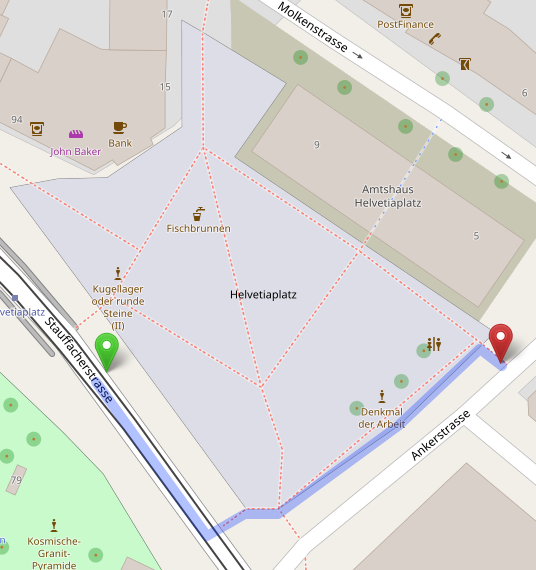
\includegraphics[width=0.5\linewidth]{technicalreport/img/helvetiaplatz_graphhopper}
	\caption[Fussgänger-Routing]{Fussgänger-Routing mit GraphHopper über den Helvetiaplatz, Zürich, Schweiz; Screenshot von openstreetmap.org aufgenommen am 08.10.2017}
	\label{fig:helvetiaplatz_graphhopper}
\end{figure}

\subsubsection{eingezeichnete Fussgängerrouten über offene Flächen}
\label{problem:eingezeichnete Fussgängerrouten über offene Flächen}
Wenn man die gleiche Abbildung \ref{fig:helvetiaplatz_graphhopper} nochmals betrachtet, sieht man, dass Mapper bereits einige Fussgängerwege auf dem Platz eingezeichnet haben, um dem Routing-Problem über offene Fläche entgegen zu steuern. Dies kann in einigen Situationen wie dem Helvetiaplatz kontraproduktiv, aber in anderen wieder von Vorteil sein. Betrachtet man beispielsweise den Central Park in New York in Abbildung \ref{fig:central_park} macht es Sinn, dass das Routing den vorgegeben Wegen folgt. Eine Wiese gilt als offene Fläche, eignet sich aber nicht immer als vorteilhafter Bewegungsuntergrund. Man muss abklären, in welchen Situation man sich auf vorhandene Wege über offene Flächen verlassen kann und wann sie zu ignorieren sind. Es gilt zu prüfen, ob diese Abgrenzung mit den gegebenen Informationen überhaupt möglich ist.

\begin{figure}[ht]
\centering
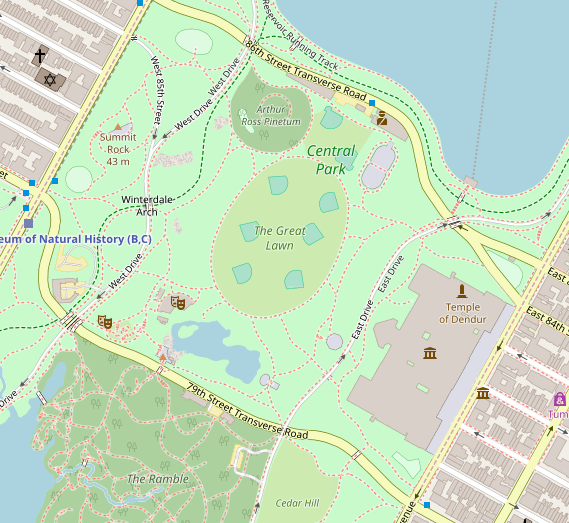
\includegraphics[width=0.5\linewidth]{technicalreport/img/central_park}
\caption[eingezeichnete Fussgänger-Routen]{Eingezeichnete Fussgänger-Routen auf dem Central Park, New York City, USA; Screenshot von openstreetmap.org aufgenommen am 08.10.2017}
\label{fig:central_park}
\end{figure}

\subsubsection{topologisch nicht verbundene Wege}
\label{problem:topologisch nicht verbundene Wege}

\begin{figure}[ht]
\centering
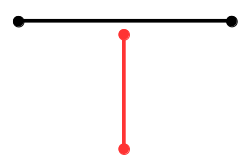
\includegraphics[width=0.5\linewidth]{technicalreport/img/topologisch_nicht_verbundener_graph}
\caption[topologisch nicht verbundener Graph]{topologisch nicht verbundener Graph}
\label{fig:topologisch_nicht_verbundener_graph}
\end{figure}

In Abbildung \ref{fig:topologisch_nicht_verbundener_graph} ist ein topologisch nicht verbundener Graph zu sehen. In \ac{OSM} kann es vorkommen, dass solche Wege auf eine offene Fläche treffen, mit dieser aber nicht topologisch verbunden sind. Eine Routing-Engine muss in der Lage sein, dies zu erkennen und aufzuräumen, so dass vom auftreffenden Weg über die offene Fläche geroutet werden kann.

\subsubsection{Routing über über weitere Arten von offenen Flächen (Berge, Strände)}
\label{problem:Routing über über weitere Arten von offenen Flächen (Berge, Strände)}
Berge und Strände sind bekanntermassen schwieriger zu überqueren als normale Plätze. Sei dies aufgrund der zurückzulegenden Höhendifferenz oder die Unterlage, welche das Fortbewegen mühsamer macht. Zusätzlich zum Problem \ref{problem:Routing über offene Flächen} kommt hier dazu, dass Umlaufen dieser offenen Flächen (Berge, Strände) effizienter sein kann als das Überqueren.

\subsubsection{Start-/Endpunkt auf der Fläche}
\label{problem:Start-/Endpunkt auf der Fläche}
Beginnt das Routing oder ist der Zielort auf einer Fläche, so ziehen die aktuellen Routing-Engines, falls keine Wege wie in \ref{problem:eingezeichnete Fussgängerrouten über offene Flächen} beschrieben eingezeichnet sind, eine rechtwinklige Linie zur nächsten Kante der Fläche und routen von dort weiter. Dies ist gut auf dem Sechseläutenplatz in Abbildung \ref{fig:start_endpoint_on_area} sichtbar. Falls bereits Wege auf der Fläche eingezeichnet sind, wird über diese geroutet.

\begin{figure}[ht]
    \centering
    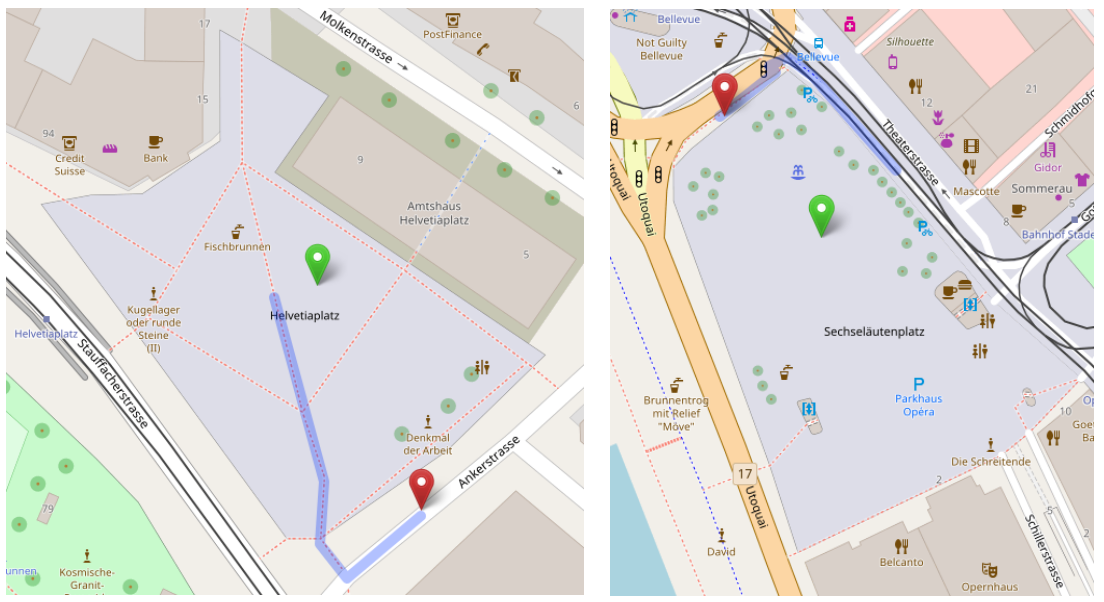
\includegraphics[width=1\linewidth]{technicalreport/img/start_endpoint_on_area}
    \caption[Fussgänger-Routing mit Startpunkt auf der Fläche]{Fussgänger-Routing mit GraphHopper über den Helvetiaplatz (links) und Sechseläutenplatz (rechts), Zürich, Schweiz mit Startpunkt auf der Fläche; Screenshot von openstreetmap.org aufgenommen am 14.10.2017}
    \label{fig:start_endpoint_on_area}
\end{figure}

\subsubsection{Routing bei zwei benachbarten Flächen}
\label{problem:Routing bei zwei benachbarten Flächen}
Es kann vorkommen, dass zwei Flächen unmittelbar nebeneinander liegen. Dies ist beim Bundesplatz in Bern, Schweiz der Fall, welcher direkt an den Bärenplatz grenzt. Dies ist in Abbildung \ref{fig:bundesplatz_baerenplatz} sichtbar. Das erschwert das Routing über Flächen, da nicht direkt Entry-Points eines Polygons genutzt werden können.

\begin{figure}[ht]
\centering
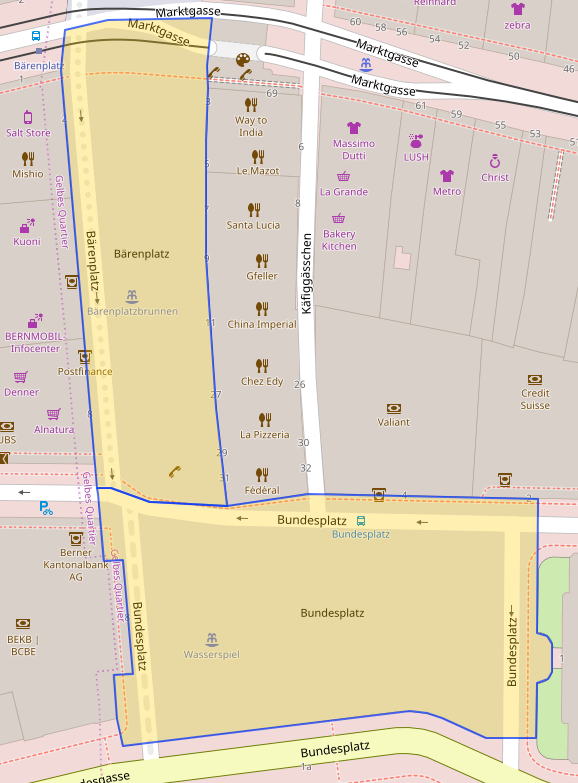
\includegraphics[width=0.5\linewidth]{technicalreport/img/bundesplatz_baerenplatz}
\caption[Zwei benachbarte Flächen]{Zwei benachbarte Flächen (Bundesplatz, Bärenplatz) in Bern, Schweiz; Screenshot von overpass-turbo.eu aufgenommen am 18.10.2017}
\label{fig:bundesplatz_baerenplatz}
\end{figure}

\subsubsection{mehrere ÖV-Stationen mit dem gleichen Namen}
\label{problem:mehrere ÖV-Stationen mit dem gleichen Namen}
In den meisten Fällen gibt es an einem Standort mit einer ÖV-Station zwei Stationen mit dem gleichen Namen, je eine für die jeweilige Fahrtrichtung. In manchen Fällen ist es so, dass diese Stationen ein Stück voneinander entfernt liegen. Die Entscheidung zur welchen ÖV-Station geroutet wird, muss getroffen werden.
	
\subsection{Ziele und Unterziele}
\label{Ziele und Unterziele}

\subsubsection{Routing über offene Flächen}
\label{target:Routing über offene Flächen}
Das Problem wie in \ref{problem:Routing über offene Flächen} beschrieben wurde bereits in einigen Arbeiten aufgegriffen \cite{graser_visibility_graph}, \cite{dzafic_spider_web_graph}. Diese beiden Ansätze (Visibility-Graph und SpiderWeb-Graph) werden analysiert, Tests in QGIS implementiert und getestet. Ziel ist es, die optimale Variante zu eruieren, um über offene Flächen den schnellstmöglichen Weg zu finden.

\subsubsection{Routing-Engine evaluieren}
\label{target:Routing-Enginge evaluieren}
Die zahlreichen Routing-Engines sollen analysiert und festgehalten werden, welche sich für den Hauptzweck dieser Arbeit am besten eignet. Zusätzlich wird geprüft, wie die Datenvorverarbeitung (Einzeichnen der Routen für Routing über offene Flächen) in die bestehenden Routing-Engines eingehängt werden kann.

\subsubsection{eingezeichnete Fussgängerrouten über offene Flächen}
\label{target:eingezeichnete Fussgängerrouten über offene Flächen}
Es soll eruiert werden, ob für den Platz die eingezeichneten Fussgängerrouten ignoriert werden können oder ob man an diese gebunden ist, wie man in Abbildung \ref{fig:central_park} sieht.

\subsubsection{topologisch nicht verbundene Wege}
\label{target:topologisch nicht verbundene Wege}
Dieses Problem ist der Vollständigkeit halber aufgeführt, wird in dieser Arbeit aber nicht weiter verfolgt.
%TODO bereits Teil der Routing-Engines

\subsubsection{Routing über über weitere Arten von offenen Flächen (Berge, Strände)}
\label{target:Routing über über weitere Arten von offenen Flächen (Berge, Strände)}
Im Kontext dieser Arbeit wird kurz ein theoretischer Ansatz aufgezeigt, wie man mit einem kostenbasierten Graph den Eigenschaften diesen Unterflächen gerecht werden könnte.

\subsubsection{Start-/Endpunkt auf der Fläche}
\label{target:Start-/Endpunkt auf der Fläche}
Der Start des Fussgänger-Routing ist von überall möglich. Somit soll es möglich sein, dass das Routing auf einer Fläche beginnen kann und man nicht wie in \ref{problem:Start-/Endpunkt auf der Fläche} beschrieben, zur nächstgelegenen Polygonkante geroutet wird. Es soll geklärt werden, ob die Vorverarbeitung der Flächen, wie es in \ref{target:Routing über offene Flächen} vorgesehen ist, ausreicht, oder ob zu einem späteren Zeitpunkt ein Echtzeit-Verarbeitung der Fläche vom aktuellen Standort aus in Betracht gezogen werden muss.

\subsubsection{Routing bei zwei benachbarten Flächen}
\label{target:Routing bei zwei benachbarten Flächen}
Dieses Problem ist der Vollständigkeit halber aufgeführt, wird in dieser Arbeit aber nicht weiter verfolgt.

\subsubsection{nächste ÖV-Haltestellen finden}
\label{target:nächste ÖV-Haltestellen finden}
Der Fokus der Arbeit liegt auf dem Finden und Erreichen der nächsten ÖV-Haltestelle, welche einem ans gewünschte Ziel führt. So soll eruiert werden, wie von einem bestehenden Startpunkt aus die nächsten ÖV-Haltestellen identifiziert werden, um diese an search.ch für das weitere Routing zu übergeben.

\subsubsection{mehrere ÖV-Stationen mit dem gleichen Namen}
\label{target:mehrere ÖV-Stationen mit dem gleichen Namen}
Wurde die nächste Haltestelle wie in \ref{target:nächste ÖV-Haltestellen finden} beschrieben, eruiert, so gilt es zur ÖV-Station in die richtige Fahrtrichtung zu routen.

\subsubsection{Prototyp und Deliverables}
\label{target:Prototyp und Deliverables}
Das Resultat besteht aus zwei Teilen. Einerseits wird es möglich sein, \ac{OSM}-Daten vorzuverarbeiten, um das Fussgänger-Routing im urbanen Raum sicherzustellen. In einem weiteren Schritt wird die Vorverarbeitung in einem Prototyp sichtbar gemacht. Dieser besteht aus einem Routing-Service mit einem QGIS-Plugin als Frontend, welcher das Zusammenspiel zwischen dem Fussgänger-Routing und der search.ch-\ac{API} aufzeigt. Die detaillierten Anforderungen an den Prototyp sind im Kapitel \ref{sec:Anforderungsspezifikation} beschrieben.
	
\subsection{Rahmenbedingungen, Umfeld, Definitionen, Abgrenzungen}
\label{Rahmenbedingungen, Umfeld, Definitionen, Abgrenzungen}
Die Arbeit befasst sich mit Flächen im urbanen Raum. Berge, Strände, Parks, etc. werden bewusst ausgeklammert, um nicht den Rahmen der Arbeit zu sprengen. Voraussetzung ist, dass Python als Programmiersprache verwendet wird und \ac{OSM}-Daten \cite{osm_data_switzerland} verarbeitet werden.

Als Drittsysteme sind die \ac{API} von search.ch \cite{search_ch_route_api} für das ÖV-Routing und Overpass \cite{wiki:overpass} für das Extrahieren von spezifischen \ac{OSM}-Daten zu gebrauchen.

Die Backend-Komponente sollen als Docker-Container für eine einfache Portierung verfügbar sein. Die Funktionalität der Komponenten werden kontinuierlich mit Continuous Integration sichergestellt.

\subsection{Vorgehen und Aufbau der Arbeit}
\label{Vorgehen und Aufbau der Arbeit}
Die Studienarbeit nimmt sich zu erst dem Problem des Fussgänger-Routing über Flächen im urbanen Raum an. Es wird geklärt, wie momentan die Thematik gehandhabt wird und welche Vorarbeiten und Lösungen in diesem Bereich existieren. Bestehende Lösungsvorschläge werden mit der Hilfe von QGIS in Python implementiert, um so die bestmögliche Variante zu eruieren. Das gleiche Vorgehen wird für das Fussgänger-Routing über Strassen gewählt. Sobald die bestmöglichen Lösungsvarianten identifiziert sind, muss geklärt werden, wie die Vorverarbeitung der Daten (beispielsweise, das Einzeichnen von möglichen Routen über Flächen) an eine bestehende Routing-Engine übergeben werden kann. Damit dies möglich ist, ist zu prüfen, welche Engine die Anforderungen bestmöglich abdecken.

In einem weiteren Schritt soll ermittelt werden, wie die nächsten ÖV-Haltestellen eruiert werden können, um diese Punkte an die API von search.ch übergeben zu können. Aufgabe von search.ch ist es, für n Startpunkte die ÖV-Route zu genieren. So ist es möglich, denn schnellstmöglichen Weg für eine Route in Kombination von Fussweg und öffentlichem Weg zu ermitteln.

Die vorhin aufgeführten Aspekte werden im Kapitel \ref{chap:Technischer Bericht} behandelt.

In einem zweiten Teil werden die im Teil 1 erarbeiteten Artefakte zusammengeführt. Es wird in QGIS ein Prototyp implementiert. Die Ergebnisse werden im Kapitel \ref{chap:SW-Projektdokumentation} beschrieben.

% TODO wie sieht Prototyp genau aus


% TODO Grafik mit Epics und einigen Unterpunkten was dazu gehört

\subsection{Grundlagen und Begriffe}
\label{Grundlagen und Begriffe}

Im folgenden werden einige theoretische Grundlagen und Begriffe eingeführt, welche im Laufe des Dokuments auftauchen werden.

% TODO was muss alles noch eingeführt werden?


\subsubsection{Fläche}
\label{Fläche}

Als Fläche werden für diesen Zweck Plätze, Wiesen, etc. verstanden, die von Fussgänger frei begehbar sind. Flächen sind in \ac{OSM} keine eigenständige Datenelemente. Es handelt sich dabei um Polygone (sprich geschlossene Linien) oder Multipolygone (siehe \ref{Multipolygon}), welche in \ac{OSM} mit den Attributen \textit{landuse=*} oder mit \textit{highway=footway} und \textit{area=yes} versehen sind. Fehlt \textit{area=yes} wird die geschlossene Linie als Rundweg interpretiert, über welche nicht geroutet werden soll. \cite{osm_wiki_area}
% TODO: Wie genau filtern wir nach Flächen? Area=yes UND highway=pedestrian?

\subsubsection{nicht-motorisierter Individualverkehr}
\label{nicht-motorisierter Individualverkehr}

Zum nicht-motorisierten Individualverkehr gehören unter anderem Fussgänger, Rollstuhlfahrer und Radfahrer.

Zur besseren Lesbarkeit und der Einfachheit halber wird in der Arbeit nur noch von Fussgänger gesprochen.

\subsubsection{Multipolygon}
\label{Multipolygon}

Multipolygone in \ac{OSM} sind ein oder mehrere Polygone, die jeweils einen geschlossenen Pfad beschreiben. Jedes Polygon kann entweder als einen äusseren oder inneren Ring dienen. So kann ein innerer Ring eine Teilfläche eines äusseren Rings ausschneiden. Polygone in einem Multipolygon können auch disjunkt sein. \cite{osm_wiki_multipolygon}

\begin{figure}[th]
\centering
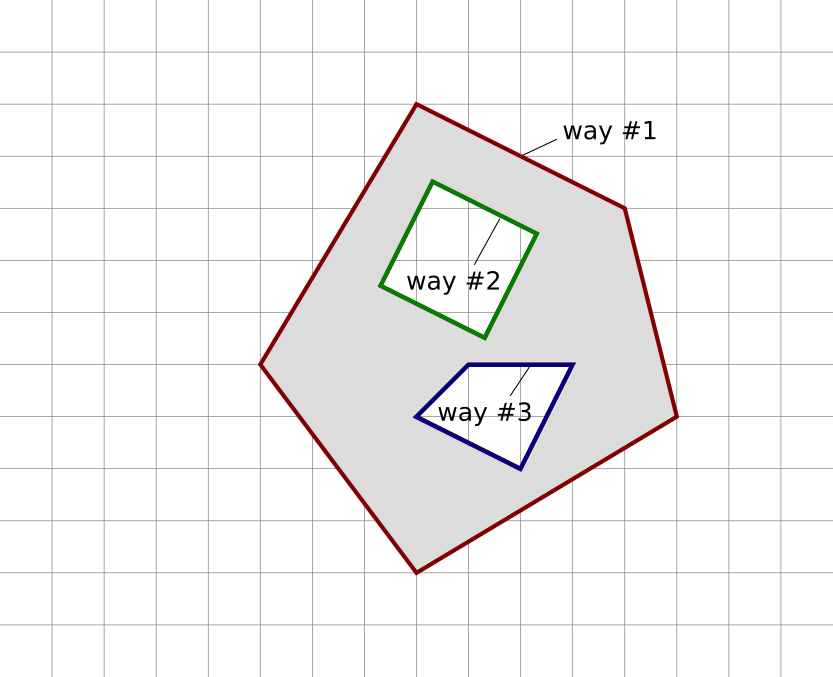
\includegraphics[width=0.5\linewidth]{technicalreport/img/multipolygon_osm_example.png}
\caption[Multipolygon OSM Example]{Beispiel eines Multipolygons in \ac{OSM} mit einem äusseren und zwei inneren Ringen. \cite{osm_wiki_multipolygon}}
\label{fig:multipolygon_osm_example}
\end{figure}

In GIS hingegen ist ein Multipolygon definiert als mehrere sich nicht überschneidende Polygone. Jedes Polygon wird durch ein oder mehrere geschlossene Pfade beschrieben. Dabei ist der erste Pfad der äussere Rand, alle weiteren Pfade beschreiben innere Ringe. \cite{opengis_simple_features}

\subsubsection{Hindernisse auf Flächen}
\label{Hindernisse in Flächen}

TODO % wie sieht Datenstruktur aus


\subsubsection{Shortest Path}
\label{Shortest Path}

TODO
